\documentclass[1p]{elsarticle_modified}
%\bibliographystyle{elsarticle-num}

%\usepackage[colorlinks]{hyperref}
%\usepackage{abbrmath_seonhwa} %\Abb, \Ascr, \Acal ,\Abf, \Afrak
\usepackage{amsfonts}
\usepackage{amssymb}
\usepackage{amsmath}
\usepackage{amsthm}
\usepackage{scalefnt}
\usepackage{amsbsy}
\usepackage{kotex}
\usepackage{caption}
\usepackage{subfig}
\usepackage{color}
\usepackage{graphicx}
\usepackage{xcolor} %% white, black, red, green, blue, cyan, magenta, yellow
\usepackage{float}
\usepackage{setspace}
\usepackage{hyperref}

\usepackage{tikz}
\usetikzlibrary{arrows}

\usepackage{multirow}
\usepackage{array} % fixed length table
\usepackage{hhline}

%%%%%%%%%%%%%%%%%%%%%
\makeatletter
\renewcommand*\env@matrix[1][\arraystretch]{%
	\edef\arraystretch{#1}%
	\hskip -\arraycolsep
	\let\@ifnextchar\new@ifnextchar
	\array{*\c@MaxMatrixCols c}}
\makeatother %https://tex.stackexchange.com/questions/14071/how-can-i-increase-the-line-spacing-in-a-matrix
%%%%%%%%%%%%%%%

\usepackage[normalem]{ulem}

\newcommand{\msout}[1]{\ifmmode\text{\sout{\ensuremath{#1}}}\else\sout{#1}\fi}
%SOURCE: \msout is \stkout macro in https://tex.stackexchange.com/questions/20609/strikeout-in-math-mode

\newcommand{\cancel}[1]{
	\ifmmode
	{\color{red}\msout{#1}}
	\else
	{\color{red}\sout{#1}}
	\fi
}

\newcommand{\add}[1]{
	{\color{blue}\uwave{#1}}
}

\newcommand{\replace}[2]{
	\ifmmode
	{\color{red}\msout{#1}}{\color{blue}\uwave{#2}}
	\else
	{\color{red}\sout{#1}}{\color{blue}\uwave{#2}}
	\fi
}

\newcommand{\Sol}{\mathcal{S}} %segment
\newcommand{\D}{D} %diagram
\newcommand{\A}{\mathcal{A}} %arc


%%%%%%%%%%%%%%%%%%%%%%%%%%%%%5 test

\def\sl{\operatorname{\textup{SL}}(2,\Cbb)}
\def\psl{\operatorname{\textup{PSL}}(2,\Cbb)}
\def\quan{\mkern 1mu \triangleright \mkern 1mu}

\theoremstyle{definition}
\newtheorem{thm}{Theorem}[section]
\newtheorem{prop}[thm]{Proposition}
\newtheorem{lem}[thm]{Lemma}
\newtheorem{ques}[thm]{Question}
\newtheorem{cor}[thm]{Corollary}
\newtheorem{defn}[thm]{Definition}
\newtheorem{exam}[thm]{Example}
\newtheorem{rmk}[thm]{Remark}
\newtheorem{alg}[thm]{Algorithm}

\newcommand{\I}{\sqrt{-1}}
\begin{document}

%\begin{frontmatter}
%
%\title{Boundary parabolic representations of knots up to 8 crossings}
%
%%% Group authors per affiliation:
%\author{Yunhi Cho} 
%\address{Department of Mathematics, University of Seoul, Seoul, Korea}
%\ead{yhcho@uos.ac.kr}
%
%
%\author{Seonhwa Kim} %\fnref{s_kim}}
%\address{Center for Geometry and Physics, Institute for Basic Science, Pohang, 37673, Korea}
%\ead{ryeona17@ibs.re.kr}
%
%\author{Hyuk Kim}
%\address{Department of Mathematical Sciences, Seoul National University, Seoul 08826, Korea}
%\ead{hyukkim@snu.ac.kr}
%
%\author{Seokbeom Yoon}
%\address{Department of Mathematical Sciences, Seoul National University, Seoul, 08826,  Korea}
%\ead{sbyoon15@snu.ac.kr}
%
%\begin{abstract}
%We find all boundary parabolic representation of knots up to 8 crossings.
%
%\end{abstract}
%\begin{keyword}
%    \MSC[2010] 57M25 
%\end{keyword}
%
%\end{frontmatter}

%\linenumbers
%\tableofcontents
%
\newcommand\colored[1]{\textcolor{white}{\rule[-0.35ex]{0.8em}{1.4ex}}\kern-0.8em\color{red} #1}%
%\newcommand\colored[1]{\textcolor{white}{ #1}\kern-2.17ex	\textcolor{white}{ #1}\kern-1.81ex	\textcolor{white}{ #1}\kern-2.15ex\color{red}#1	}

{\Large $\underline{12a_{0377}~(K12a_{0377})}$}

\setlength{\tabcolsep}{10pt}
\renewcommand{\arraystretch}{1.6}
\vspace{1cm}\begin{tabular}{m{100pt}>{\centering\arraybackslash}m{274pt}}
\multirow{5}{120pt}{
	\centering
	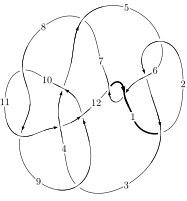
\includegraphics[width=112pt]{../../../GIT/diagram.site/Diagrams/png/1178_12a_0377.png}\\
\ \ \ A knot diagram\footnotemark}&
\allowdisplaybreaks
\textbf{Linearized knot diagam} \\
\cline{2-2}
 &
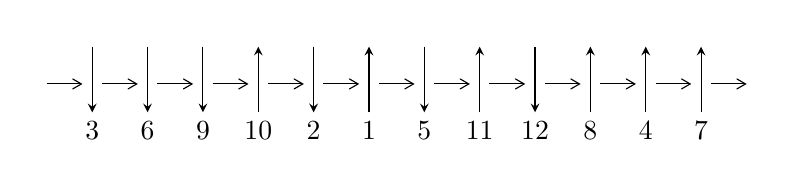
\begin{tikzpicture}[x=20pt, y=17pt]
	% nodes
	\node (C0) at (0, 0) {};
	\node (C1) at (1, 0) {};
	\node (C1U) at (1, +1) {};
	\node (C1D) at (1, -1) {3};

	\node (C2) at (2, 0) {};
	\node (C2U) at (2, +1) {};
	\node (C2D) at (2, -1) {6};

	\node (C3) at (3, 0) {};
	\node (C3U) at (3, +1) {};
	\node (C3D) at (3, -1) {9};

	\node (C4) at (4, 0) {};
	\node (C4U) at (4, +1) {};
	\node (C4D) at (4, -1) {10};

	\node (C5) at (5, 0) {};
	\node (C5U) at (5, +1) {};
	\node (C5D) at (5, -1) {2};

	\node (C6) at (6, 0) {};
	\node (C6U) at (6, +1) {};
	\node (C6D) at (6, -1) {1};

	\node (C7) at (7, 0) {};
	\node (C7U) at (7, +1) {};
	\node (C7D) at (7, -1) {5};

	\node (C8) at (8, 0) {};
	\node (C8U) at (8, +1) {};
	\node (C8D) at (8, -1) {11};

	\node (C9) at (9, 0) {};
	\node (C9U) at (9, +1) {};
	\node (C9D) at (9, -1) {12};

	\node (C10) at (10, 0) {};
	\node (C10U) at (10, +1) {};
	\node (C10D) at (10, -1) {8};

	\node (C11) at (11, 0) {};
	\node (C11U) at (11, +1) {};
	\node (C11D) at (11, -1) {4};

	\node (C12) at (12, 0) {};
	\node (C12U) at (12, +1) {};
	\node (C12D) at (12, -1) {7};
	\node (C13) at (13, 0) {};

	% arrows
	\draw[->,>={angle 60}]
	(C0) edge (C1) (C1) edge (C2) (C2) edge (C3) (C3) edge (C4) (C4) edge (C5) (C5) edge (C6) (C6) edge (C7) (C7) edge (C8) (C8) edge (C9) (C9) edge (C10) (C10) edge (C11) (C11) edge (C12) (C12) edge (C13) ;	\draw[->,>=stealth]
	(C1U) edge (C1D) (C2U) edge (C2D) (C3U) edge (C3D) (C4D) edge (C4U) (C5U) edge (C5D) (C6D) edge (C6U) (C7U) edge (C7D) (C8D) edge (C8U) (C9U) edge (C9D) (C10D) edge (C10U) (C11D) edge (C11U) (C12D) edge (C12U) ;
	\end{tikzpicture} \\
\hhline{~~} \\& 
\textbf{Solving Sequence} \\ \cline{2-2} 
 &
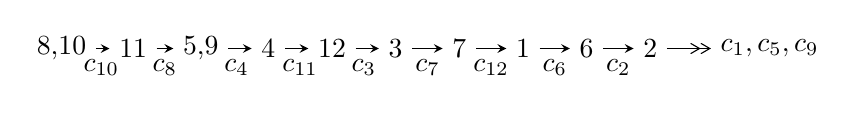
\begin{tikzpicture}[x=23pt, y=7pt]
	% node
	\node (A0) at (-1/8, 0) {8,10};
	\node (A1) at (1, 0) {11};
	\node (A2) at (33/16, 0) {5,9};
	\node (A3) at (25/8, 0) {4};
	\node (A4) at (33/8, 0) {12};
	\node (A5) at (41/8, 0) {3};
	\node (A6) at (49/8, 0) {7};
	\node (A7) at (57/8, 0) {1};
	\node (A8) at (65/8, 0) {6};
	\node (A9) at (73/8, 0) {2};
	\node (C1) at (1/2, -1) {$c_{10}$};
	\node (C2) at (3/2, -1) {$c_{8}$};
	\node (C3) at (21/8, -1) {$c_{4}$};
	\node (C4) at (29/8, -1) {$c_{11}$};
	\node (C5) at (37/8, -1) {$c_{3}$};
	\node (C6) at (45/8, -1) {$c_{7}$};
	\node (C7) at (53/8, -1) {$c_{12}$};
	\node (C8) at (61/8, -1) {$c_{6}$};
	\node (C9) at (69/8, -1) {$c_{2}$};
	\node (A10) at (11, 0) {$c_{1},c_{5},c_{9}$};

	% edge
	\draw[->,>=stealth]	
	(A0) edge (A1) (A1) edge (A2) (A2) edge (A3) (A3) edge (A4) (A4) edge (A5) (A5) edge (A6) (A6) edge (A7) (A7) edge (A8) (A8) edge (A9) ;
	\draw[->>,>={angle 60}]	
	(A9) edge (A10);
\end{tikzpicture} \\ 

\end{tabular} \\

\footnotetext{
The image of knot diagram is generated by the software ``\textbf{Draw programme}" developed by Andrew Bartholomew(\url{http://www.layer8.co.uk/maths/draw/index.htm\#Running-draw}), where we modified some parts for our purpose(\url{https://github.com/CATsTAILs/LinksPainter}).
}\phantom \\ \newline 
\centering \textbf{Ideals for irreducible components\footnotemark of $X_{\text{par}}$} 
 
\begin{align*}
I^u_{1}&=\langle 
3.60458\times10^{351} u^{112}-1.49802\times10^{352} u^{111}+\cdots+1.58423\times10^{352} b+8.96032\times10^{351},\\
\phantom{I^u_{1}}&\phantom{= \langle  }3.98283\times10^{351} u^{112}-1.51474\times10^{352} u^{111}+\cdots+1.58423\times10^{352} a-6.48283\times10^{352},\;u^{113}+2 u^{112}+\cdots+5 u+1\rangle \\
I^u_{2}&=\langle 
b+1,\;a-1,\;u-1\rangle \\
\\
\end{align*}
\raggedright * 2 irreducible components of $\dim_{\mathbb{C}}=0$, with total 114 representations.\\
\footnotetext{All coefficients of polynomials are rational numbers. But the coefficients are sometimes approximated in decimal forms when there is not enough margin.}
\newpage
\renewcommand{\arraystretch}{1}
\centering \section*{I. $I^u_{1}= \langle 3.60\times10^{351} u^{112}-1.50\times10^{352} u^{111}+\cdots+1.58\times10^{352} b+8.96\times10^{351},\;3.98\times10^{351} u^{112}-1.51\times10^{352} u^{111}+\cdots+1.58\times10^{352} a-6.48\times10^{352},\;u^{113}+2 u^{112}+\cdots+5 u+1 \rangle$}
\flushleft \textbf{(i) Arc colorings}\\
\begin{tabular}{m{7pt} m{180pt} m{7pt} m{180pt} }
\flushright $a_{8}=$&$\begin{pmatrix}0\\u\end{pmatrix}$ \\
\flushright $a_{10}=$&$\begin{pmatrix}1\\0\end{pmatrix}$ \\
\flushright $a_{11}=$&$\begin{pmatrix}1\\- u^2\end{pmatrix}$ \\
\flushright $a_{5}=$&$\begin{pmatrix}-0.251405 u^{112}+0.956139 u^{111}+\cdots-51.3075 u+4.09211\\-0.227529 u^{112}+0.945582 u^{111}+\cdots-6.03599 u-0.565596\end{pmatrix}$ \\
\flushright $a_{9}=$&$\begin{pmatrix}u\\- u^3+u\end{pmatrix}$ \\
\flushright $a_{4}=$&$\begin{pmatrix}-0.0238759 u^{112}+0.0105577 u^{111}+\cdots-45.2715 u+4.65770\\-0.227529 u^{112}+0.945582 u^{111}+\cdots-6.03599 u-0.565596\end{pmatrix}$ \\
\flushright $a_{12}=$&$\begin{pmatrix}3.74173 u^{112}+1.87309 u^{111}+\cdots+31.7286 u+1.20630\\-1.57162 u^{112}-1.04502 u^{111}+\cdots-6.80780 u-1.86865\end{pmatrix}$ \\
\flushright $a_{3}=$&$\begin{pmatrix}-0.601635 u^{112}+0.284080 u^{111}+\cdots-50.9813 u+3.32938\\0.267924 u^{112}+1.62204 u^{111}+\cdots-5.17838 u-0.464880\end{pmatrix}$ \\
\flushright $a_{7}=$&$\begin{pmatrix}0.925335 u^{112}+0.0971187 u^{111}+\cdots+20.9526 u-4.66114\\-1.77138 u^{112}-1.42443 u^{111}+\cdots-3.14980 u-1.70177\end{pmatrix}$ \\
\flushright $a_{1}=$&$\begin{pmatrix}-0.155973 u^{112}-1.13087 u^{111}+\cdots+31.7267 u-2.05511\\0.479124 u^{112}+0.772006 u^{111}+\cdots-0.580322 u-0.354009\end{pmatrix}$ \\
\flushright $a_{6}=$&$\begin{pmatrix}-1.60565 u^{112}-1.74713 u^{111}+\cdots+15.2116 u-7.47774\\-1.73965 u^{112}-1.54559 u^{111}+\cdots-1.04522 u-1.46991\end{pmatrix}$ \\
\flushright $a_{2}=$&$\begin{pmatrix}0.273879 u^{112}-0.0294619 u^{111}+\cdots+5.15495 u+3.64220\\1.52493 u^{112}+1.56504 u^{111}+\cdots+1.07514 u+0.790347\end{pmatrix}$\\&\end{tabular}
\flushleft \textbf{(ii) Obstruction class $= -1$}\\~\\
\flushleft \textbf{(iii) Cusp Shapes $= -9.37846 u^{112}-6.07388 u^{111}+\cdots+8.52876 u-10.5678$}\\~\\
\newpage\renewcommand{\arraystretch}{1}
\flushleft \textbf{(iv) u-Polynomials at the component}\newline \\
\begin{tabular}{m{50pt}|m{274pt}}
Crossings & \hspace{64pt}u-Polynomials at each crossing \\
\hline $$\begin{aligned}c_{1}\end{aligned}$$&$\begin{aligned}
&u^{113}+60 u^{112}+\cdots+5 u+1
\end{aligned}$\\
\hline $$\begin{aligned}c_{2},c_{5}\end{aligned}$$&$\begin{aligned}
&u^{113}+2 u^{112}+\cdots- u+1
\end{aligned}$\\
\hline $$\begin{aligned}c_{3}\end{aligned}$$&$\begin{aligned}
&u^{113}+66 u^{111}+\cdots-5294 u+11036
\end{aligned}$\\
\hline $$\begin{aligned}c_{4}\end{aligned}$$&$\begin{aligned}
&u^{113}+2 u^{112}+\cdots+779133 u+135659
\end{aligned}$\\
\hline $$\begin{aligned}c_{6},c_{12}\end{aligned}$$&$\begin{aligned}
&u^{113}+3 u^{112}+\cdots+1248 u+288
\end{aligned}$\\
\hline $$\begin{aligned}c_{7}\end{aligned}$$&$\begin{aligned}
&u^{113}-10 u^{112}+\cdots+170569 u+7433
\end{aligned}$\\
\hline $$\begin{aligned}c_{8},c_{10}\end{aligned}$$&$\begin{aligned}
&u^{113}+2 u^{112}+\cdots+5 u+1
\end{aligned}$\\
\hline $$\begin{aligned}c_{9}\end{aligned}$$&$\begin{aligned}
&u^{113}-19 u^{112}+\cdots+6 u-2
\end{aligned}$\\
\hline $$\begin{aligned}c_{11}\end{aligned}$$&$\begin{aligned}
&u^{113}-2 u^{112}+\cdots- u+1
\end{aligned}$\\
\hline
\end{tabular}\\~\\
\newpage\renewcommand{\arraystretch}{1}
\flushleft \textbf{(v) Riley Polynomials at the component}\newline \\
\begin{tabular}{m{50pt}|m{274pt}}
Crossings & \hspace{64pt}Riley Polynomials at each crossing \\
\hline $$\begin{aligned}c_{1}\end{aligned}$$&$\begin{aligned}
&y^{113}-12 y^{112}+\cdots+73 y-1
\end{aligned}$\\
\hline $$\begin{aligned}c_{2},c_{5}\end{aligned}$$&$\begin{aligned}
&y^{113}-60 y^{112}+\cdots+5 y-1
\end{aligned}$\\
\hline $$\begin{aligned}c_{3}\end{aligned}$$&$\begin{aligned}
&y^{113}+132 y^{112}+\cdots-7542338484 y-121793296
\end{aligned}$\\
\hline $$\begin{aligned}c_{4}\end{aligned}$$&$\begin{aligned}
&y^{113}+76 y^{112}+\cdots+814063865689 y-18403364281
\end{aligned}$\\
\hline $$\begin{aligned}c_{6},c_{12}\end{aligned}$$&$\begin{aligned}
&y^{113}+81 y^{112}+\cdots+2154816 y-82944
\end{aligned}$\\
\hline $$\begin{aligned}c_{7}\end{aligned}$$&$\begin{aligned}
&y^{113}+48 y^{112}+\cdots-12384794263 y-55249489
\end{aligned}$\\
\hline $$\begin{aligned}c_{8},c_{10}\end{aligned}$$&$\begin{aligned}
&y^{113}-80 y^{112}+\cdots+201 y-1
\end{aligned}$\\
\hline $$\begin{aligned}c_{9}\end{aligned}$$&$\begin{aligned}
&y^{113}+9 y^{112}+\cdots-64 y-4
\end{aligned}$\\
\hline $$\begin{aligned}c_{11}\end{aligned}$$&$\begin{aligned}
&y^{113}-20 y^{112}+\cdots+5 y-1
\end{aligned}$\\
\hline
\end{tabular}\\~\\
\newpage\flushleft \textbf{(vi) Complex Volumes and Cusp Shapes}
$$\begin{array}{c|c|c}  
\text{Solutions to }I^u_{1}& \I (\text{vol} + \sqrt{-1}CS) & \text{Cusp shape}\\
 \hline 
\begin{aligned}
u &= \phantom{-}0.628994 + 0.805074 I \\
a &= \phantom{-}0.469841 - 0.263890 I \\
b &= \phantom{-}0.283186 + 0.181705 I\end{aligned}
 & -2.56577 + 5.23147 I & \phantom{-0.000000 } 0 \\ \hline\begin{aligned}
u &= \phantom{-}0.628994 - 0.805074 I \\
a &= \phantom{-}0.469841 + 0.263890 I \\
b &= \phantom{-}0.283186 - 0.181705 I\end{aligned}
 & -2.56577 - 5.23147 I & \phantom{-0.000000 } 0 \\ \hline\begin{aligned}
u &= \phantom{-}0.325320 + 0.898186 I \\
a &= -0.556699 - 0.146988 I \\
b &= -0.544491 - 0.403405 I\end{aligned}
 & \phantom{-}0.61481 + 1.65437 I & \phantom{-0.000000 } 0 \\ \hline\begin{aligned}
u &= \phantom{-}0.325320 - 0.898186 I \\
a &= -0.556699 + 0.146988 I \\
b &= -0.544491 + 0.403405 I\end{aligned}
 & \phantom{-}0.61481 - 1.65437 I & \phantom{-0.000000 } 0 \\ \hline\begin{aligned}
u &= \phantom{-}0.943592 + 0.030818 I \\
a &= -0.522216 + 0.154103 I \\
b &= \phantom{-}0.68200 + 2.38604 I\end{aligned}
 & \phantom{-}0.340243 + 0.243306 I & \phantom{-0.000000 } 0 \\ \hline\begin{aligned}
u &= \phantom{-}0.943592 - 0.030818 I \\
a &= -0.522216 - 0.154103 I \\
b &= \phantom{-}0.68200 - 2.38604 I\end{aligned}
 & \phantom{-}0.340243 - 0.243306 I & \phantom{-0.000000 } 0 \\ \hline\begin{aligned}
u &= \phantom{-}1.057710 + 0.097573 I \\
a &= \phantom{-}0.579526 - 0.832827 I \\
b &= \phantom{-}0.11853 - 3.24830 I\end{aligned}
 & -2.42343 - 1.00273 I & \phantom{-0.000000 } 0 \\ \hline\begin{aligned}
u &= \phantom{-}1.057710 - 0.097573 I \\
a &= \phantom{-}0.579526 + 0.832827 I \\
b &= \phantom{-}0.11853 + 3.24830 I\end{aligned}
 & -2.42343 + 1.00273 I & \phantom{-0.000000 } 0 \\ \hline\begin{aligned}
u &= \phantom{-}0.465316 + 0.964816 I \\
a &= \phantom{-}0.665764 - 0.055613 I \\
b &= \phantom{-}0.544662 + 0.234872 I\end{aligned}
 & -2.10528 - 2.72389 I & \phantom{-0.000000 } 0 \\ \hline\begin{aligned}
u &= \phantom{-}0.465316 - 0.964816 I \\
a &= \phantom{-}0.665764 + 0.055613 I \\
b &= \phantom{-}0.544662 - 0.234872 I\end{aligned}
 & -2.10528 + 2.72389 I & \phantom{-0.000000 } 0\\
 \hline 
 \end{array}$$\newpage$$\begin{array}{c|c|c}  
\text{Solutions to }I^u_{1}& \I (\text{vol} + \sqrt{-1}CS) & \text{Cusp shape}\\
 \hline 
\begin{aligned}
u &= -0.373895 + 0.843598 I \\
a &= -0.46944 - 1.35921 I \\
b &= -0.469024 - 1.043280 I\end{aligned}
 & -7.94586 + 5.17796 I & \phantom{-0.000000 } 0 \\ \hline\begin{aligned}
u &= -0.373895 - 0.843598 I \\
a &= -0.46944 + 1.35921 I \\
b &= -0.469024 + 1.043280 I\end{aligned}
 & -7.94586 - 5.17796 I & \phantom{-0.000000 } 0 \\ \hline\begin{aligned}
u &= -0.043363 + 0.920452 I \\
a &= \phantom{-}0.565594 + 0.784941 I \\
b &= \phantom{-}0.624966 + 0.748908 I\end{aligned}
 & -2.70032 + 3.74058 I & \phantom{-0.000000 } 0 \\ \hline\begin{aligned}
u &= -0.043363 - 0.920452 I \\
a &= \phantom{-}0.565594 - 0.784941 I \\
b &= \phantom{-}0.624966 - 0.748908 I\end{aligned}
 & -2.70032 - 3.74058 I & \phantom{-0.000000 } 0 \\ \hline\begin{aligned}
u &= \phantom{-}1.079330 + 0.075300 I \\
a &= -0.440245 + 0.926018 I \\
b &= -0.09491 + 3.38127 I\end{aligned}
 & \phantom{-}1.38276 + 2.70786 I & \phantom{-0.000000 } 0 \\ \hline\begin{aligned}
u &= \phantom{-}1.079330 - 0.075300 I \\
a &= -0.440245 - 0.926018 I \\
b &= -0.09491 - 3.38127 I\end{aligned}
 & \phantom{-}1.38276 - 2.70786 I & \phantom{-0.000000 } 0 \\ \hline\begin{aligned}
u &= -1.084540 + 0.070158 I \\
a &= \phantom{-}1.48569 - 0.82488 I \\
b &= -0.540270 - 0.042016 I\end{aligned}
 & \phantom{-}0.203429 - 0.594606 I & \phantom{-0.000000 } 0 \\ \hline\begin{aligned}
u &= -1.084540 - 0.070158 I \\
a &= \phantom{-}1.48569 + 0.82488 I \\
b &= -0.540270 + 0.042016 I\end{aligned}
 & \phantom{-}0.203429 + 0.594606 I & \phantom{-0.000000 } 0 \\ \hline\begin{aligned}
u &= \phantom{-}1.091440 + 0.016134 I \\
a &= -0.095452 + 0.960345 I \\
b &= -0.01184 + 3.51911 I\end{aligned}
 & \phantom{-}3.80508 + 2.14831 I & \phantom{-0.000000 } 0 \\ \hline\begin{aligned}
u &= \phantom{-}1.091440 - 0.016134 I \\
a &= -0.095452 - 0.960345 I \\
b &= -0.01184 - 3.51911 I\end{aligned}
 & \phantom{-}3.80508 - 2.14831 I & \phantom{-0.000000 } 0\\
 \hline 
 \end{array}$$\newpage$$\begin{array}{c|c|c}  
\text{Solutions to }I^u_{1}& \I (\text{vol} + \sqrt{-1}CS) & \text{Cusp shape}\\
 \hline 
\begin{aligned}
u &= -1.018950 + 0.404204 I \\
a &= -1.47062 - 0.80723 I \\
b &= \phantom{-}0.466320 - 0.706084 I\end{aligned}
 & -5.96540 - 0.84182 I & \phantom{-0.000000 } 0 \\ \hline\begin{aligned}
u &= -1.018950 - 0.404204 I \\
a &= -1.47062 + 0.80723 I \\
b &= \phantom{-}0.466320 + 0.706084 I\end{aligned}
 & -5.96540 + 0.84182 I & \phantom{-0.000000 } 0 \\ \hline\begin{aligned}
u &= \phantom{-}1.093210 + 0.088942 I \\
a &= \phantom{-}0.502305 - 1.010920 I \\
b &= \phantom{-}0.16728 - 3.39536 I\end{aligned}
 & -1.54854 + 7.37352 I & \phantom{-0.000000 } 0 \\ \hline\begin{aligned}
u &= \phantom{-}1.093210 - 0.088942 I \\
a &= \phantom{-}0.502305 + 1.010920 I \\
b &= \phantom{-}0.16728 + 3.39536 I\end{aligned}
 & -1.54854 - 7.37352 I & \phantom{-0.000000 } 0 \\ \hline\begin{aligned}
u &= \phantom{-}0.197625 + 1.091860 I \\
a &= -0.866578 - 0.364637 I \\
b &= -0.785843 - 0.477687 I\end{aligned}
 & \phantom{-}2.22897 + 2.53204 I & \phantom{-0.000000 } 0 \\ \hline\begin{aligned}
u &= \phantom{-}0.197625 - 1.091860 I \\
a &= -0.866578 + 0.364637 I \\
b &= -0.785843 + 0.477687 I\end{aligned}
 & \phantom{-}2.22897 - 2.53204 I & \phantom{-0.000000 } 0 \\ \hline\begin{aligned}
u &= -1.097280 + 0.189897 I \\
a &= -0.39958 - 1.74478 I \\
b &= \phantom{-}0.544175 - 0.702514 I\end{aligned}
 & -2.04635 - 1.56955 I & \phantom{-0.000000 } 0 \\ \hline\begin{aligned}
u &= -1.097280 - 0.189897 I \\
a &= -0.39958 + 1.74478 I \\
b &= \phantom{-}0.544175 + 0.702514 I\end{aligned}
 & -2.04635 + 1.56955 I & \phantom{-0.000000 } 0 \\ \hline\begin{aligned}
u &= -0.435334 + 0.770110 I \\
a &= -0.37253 - 1.46521 I \\
b &= -0.374521 - 1.062230 I\end{aligned}
 & -7.77300 - 3.54516 I & \phantom{-0.000000 } 0 \\ \hline\begin{aligned}
u &= -0.435334 - 0.770110 I \\
a &= -0.37253 + 1.46521 I \\
b &= -0.374521 + 1.062230 I\end{aligned}
 & -7.77300 + 3.54516 I & \phantom{-0.000000 } 0\\
 \hline 
 \end{array}$$\newpage$$\begin{array}{c|c|c}  
\text{Solutions to }I^u_{1}& \I (\text{vol} + \sqrt{-1}CS) & \text{Cusp shape}\\
 \hline 
\begin{aligned}
u &= -0.368978 + 0.774867 I \\
a &= \phantom{-}0.362705 + 1.366110 I \\
b &= \phantom{-}0.410428 + 1.008490 I\end{aligned}
 & -4.39067 + 0.89920 I & \phantom{-0.000000 } 0 \\ \hline\begin{aligned}
u &= -0.368978 - 0.774867 I \\
a &= \phantom{-}0.362705 - 1.366110 I \\
b &= \phantom{-}0.410428 - 1.008490 I\end{aligned}
 & -4.39067 - 0.89920 I & \phantom{-0.000000 } 0 \\ \hline\begin{aligned}
u &= -1.068650 + 0.407745 I \\
a &= \phantom{-}1.29200 + 0.78651 I \\
b &= -0.577199 + 0.719807 I\end{aligned}
 & -2.22585 - 5.28549 I & \phantom{-0.000000 } 0 \\ \hline\begin{aligned}
u &= -1.068650 - 0.407745 I \\
a &= \phantom{-}1.29200 - 0.78651 I \\
b &= -0.577199 - 0.719807 I\end{aligned}
 & -2.22585 + 5.28549 I & \phantom{-0.000000 } 0 \\ \hline\begin{aligned}
u &= \phantom{-}0.142388 + 1.145910 I \\
a &= \phantom{-}0.960435 + 0.457518 I \\
b &= \phantom{-}0.860997 + 0.532401 I\end{aligned}
 & \phantom{-}1.88293 + 6.96291 I & \phantom{-0.000000 } 0 \\ \hline\begin{aligned}
u &= \phantom{-}0.142388 - 1.145910 I \\
a &= \phantom{-}0.960435 - 0.457518 I \\
b &= \phantom{-}0.860997 - 0.532401 I\end{aligned}
 & \phantom{-}1.88293 - 6.96291 I & \phantom{-0.000000 } 0 \\ \hline\begin{aligned}
u &= -1.073490 + 0.450936 I \\
a &= -1.25020 - 0.93708 I \\
b &= \phantom{-}0.582668 - 0.819628 I\end{aligned}
 & -5.75547 - 9.90220 I & \phantom{-0.000000 } 0 \\ \hline\begin{aligned}
u &= -1.073490 - 0.450936 I \\
a &= -1.25020 + 0.93708 I \\
b &= \phantom{-}0.582668 + 0.819628 I\end{aligned}
 & -5.75547 + 9.90220 I & \phantom{-0.000000 } 0 \\ \hline\begin{aligned}
u &= \phantom{-}1.069790 + 0.462990 I \\
a &= -0.161941 + 0.433741 I \\
b &= \phantom{-}0.518943 - 0.112408 I\end{aligned}
 & \phantom{-}1.40063 + 2.37957 I & \phantom{-0.000000 } 0 \\ \hline\begin{aligned}
u &= \phantom{-}1.069790 - 0.462990 I \\
a &= -0.161941 - 0.433741 I \\
b &= \phantom{-}0.518943 + 0.112408 I\end{aligned}
 & \phantom{-}1.40063 - 2.37957 I & \phantom{-0.000000 } 0\\
 \hline 
 \end{array}$$\newpage$$\begin{array}{c|c|c}  
\text{Solutions to }I^u_{1}& \I (\text{vol} + \sqrt{-1}CS) & \text{Cusp shape}\\
 \hline 
\begin{aligned}
u &= -1.150660 + 0.187578 I \\
a &= \phantom{-}0.35704 + 1.62839 I \\
b &= -0.656035 + 0.699053 I\end{aligned}
 & \phantom{-}2.32331 - 5.37707 I & \phantom{-0.000000 } 0 \\ \hline\begin{aligned}
u &= -1.150660 - 0.187578 I \\
a &= \phantom{-}0.35704 - 1.62839 I \\
b &= -0.656035 - 0.699053 I\end{aligned}
 & \phantom{-}2.32331 + 5.37707 I & \phantom{-0.000000 } 0 \\ \hline\begin{aligned}
u &= -1.160570 + 0.216923 I \\
a &= -0.29068 - 1.64577 I \\
b &= \phantom{-}0.673011 - 0.761982 I\end{aligned}
 & -0.63504 - 10.38720 I & \phantom{-0.000000 } 0 \\ \hline\begin{aligned}
u &= -1.160570 - 0.216923 I \\
a &= -0.29068 + 1.64577 I \\
b &= \phantom{-}0.673011 + 0.761982 I\end{aligned}
 & -0.63504 + 10.38720 I & \phantom{-0.000000 } 0 \\ \hline\begin{aligned}
u &= -0.007650 + 1.182640 I \\
a &= -1.028660 - 0.719034 I \\
b &= -0.919799 - 0.715399 I\end{aligned}
 & -5.18160 + 3.86014 I & \phantom{-0.000000 } 0 \\ \hline\begin{aligned}
u &= -0.007650 - 1.182640 I \\
a &= -1.028660 + 0.719034 I \\
b &= -0.919799 + 0.715399 I\end{aligned}
 & -5.18160 - 3.86014 I & \phantom{-0.000000 } 0 \\ \hline\begin{aligned}
u &= \phantom{-}0.036372 + 1.198960 I \\
a &= \phantom{-}1.056530 + 0.640937 I \\
b &= \phantom{-}0.939210 + 0.658803 I\end{aligned}
 & -1.12840 + 7.66560 I & \phantom{-0.000000 } 0 \\ \hline\begin{aligned}
u &= \phantom{-}0.036372 - 1.198960 I \\
a &= \phantom{-}1.056530 - 0.640937 I \\
b &= \phantom{-}0.939210 - 0.658803 I\end{aligned}
 & -1.12840 - 7.66560 I & \phantom{-0.000000 } 0 \\ \hline\begin{aligned}
u &= -1.200230 + 0.083318 I \\
a &= \phantom{-}0.499588 + 1.306680 I \\
b &= -0.783855 + 0.468733 I\end{aligned}
 & \phantom{-}5.81921 - 4.07245 I & \phantom{-0.000000 } 0 \\ \hline\begin{aligned}
u &= -1.200230 - 0.083318 I \\
a &= \phantom{-}0.499588 - 1.306680 I \\
b &= -0.783855 - 0.468733 I\end{aligned}
 & \phantom{-}5.81921 + 4.07245 I & \phantom{-0.000000 } 0\\
 \hline 
 \end{array}$$\newpage$$\begin{array}{c|c|c}  
\text{Solutions to }I^u_{1}& \I (\text{vol} + \sqrt{-1}CS) & \text{Cusp shape}\\
 \hline 
\begin{aligned}
u &= -1.208560 + 0.027333 I \\
a &= -0.599859 - 1.105330 I \\
b &= \phantom{-}0.817363 - 0.334604 I\end{aligned}
 & \phantom{-}6.34378 + 0.77670 I & \phantom{-0.000000 } 0 \\ \hline\begin{aligned}
u &= -1.208560 - 0.027333 I \\
a &= -0.599859 + 1.105330 I \\
b &= \phantom{-}0.817363 + 0.334604 I\end{aligned}
 & \phantom{-}6.34378 - 0.77670 I & \phantom{-0.000000 } 0 \\ \hline\begin{aligned}
u &= -1.213050 + 0.095341 I \\
a &= -0.767196 + 0.574275 I \\
b &= \phantom{-}0.866219 + 0.032953 I\end{aligned}
 & \phantom{-}4.98123 - 2.74814 I & \phantom{-0.000000 } 0 \\ \hline\begin{aligned}
u &= -1.213050 - 0.095341 I \\
a &= -0.767196 - 0.574275 I \\
b &= \phantom{-}0.866219 - 0.032953 I\end{aligned}
 & \phantom{-}4.98123 + 2.74814 I & \phantom{-0.000000 } 0 \\ \hline\begin{aligned}
u &= \phantom{-}0.028775 + 1.228150 I \\
a &= -1.108380 - 0.653518 I \\
b &= -0.977482 - 0.667107 I\end{aligned}
 & -4.11564 + 12.48680 I & \phantom{-0.000000 } 0 \\ \hline\begin{aligned}
u &= \phantom{-}0.028775 - 1.228150 I \\
a &= -1.108380 + 0.653518 I \\
b &= -0.977482 + 0.667107 I\end{aligned}
 & -4.11564 - 12.48680 I & \phantom{-0.000000 } 0 \\ \hline\begin{aligned}
u &= \phantom{-}1.242600 + 0.045176 I \\
a &= -0.0276375 - 0.0507761 I \\
b &= -1.180830 + 0.038251 I\end{aligned}
 & \phantom{-}2.42702 + 0.01183 I & \phantom{-0.000000 } 0 \\ \hline\begin{aligned}
u &= \phantom{-}1.242600 - 0.045176 I \\
a &= -0.0276375 + 0.0507761 I \\
b &= -1.180830 - 0.038251 I\end{aligned}
 & \phantom{-}2.42702 - 0.01183 I & \phantom{-0.000000 } 0 \\ \hline\begin{aligned}
u &= -1.250790 + 0.154376 I \\
a &= \phantom{-}0.634697 - 0.293779 I \\
b &= -0.976609 + 0.100492 I\end{aligned}
 & \phantom{-}2.91293 - 7.47396 I & \phantom{-0.000000 } 0 \\ \hline\begin{aligned}
u &= -1.250790 - 0.154376 I \\
a &= \phantom{-}0.634697 + 0.293779 I \\
b &= -0.976609 - 0.100492 I\end{aligned}
 & \phantom{-}2.91293 + 7.47396 I & \phantom{-0.000000 } 0\\
 \hline 
 \end{array}$$\newpage$$\begin{array}{c|c|c}  
\text{Solutions to }I^u_{1}& \I (\text{vol} + \sqrt{-1}CS) & \text{Cusp shape}\\
 \hline 
\begin{aligned}
u &= \phantom{-}0.701259 + 0.144851 I \\
a &= \phantom{-}1.144400 + 0.459612 I \\
b &= \phantom{-}0.49489 - 1.53937 I\end{aligned}
 & -3.24230 + 2.05640 I & \phantom{-0.000000 } 0 \\ \hline\begin{aligned}
u &= \phantom{-}0.701259 - 0.144851 I \\
a &= \phantom{-}1.144400 - 0.459612 I \\
b &= \phantom{-}0.49489 + 1.53937 I\end{aligned}
 & -3.24230 - 2.05640 I & \phantom{-0.000000 } 0 \\ \hline\begin{aligned}
u &= \phantom{-}0.440662 + 0.462304 I \\
a &= -0.046408 + 0.267922 I \\
b &= -0.213264 - 0.552181 I\end{aligned}
 & \phantom{-}0.42820 + 1.49790 I & \phantom{-}2.53334 - 4.59564 I \\ \hline\begin{aligned}
u &= \phantom{-}0.440662 - 0.462304 I \\
a &= -0.046408 - 0.267922 I \\
b &= -0.213264 + 0.552181 I\end{aligned}
 & \phantom{-}0.42820 - 1.49790 I & \phantom{-}2.53334 + 4.59564 I \\ \hline\begin{aligned}
u &= \phantom{-}0.588990 + 0.202664 I \\
a &= \phantom{-}1.36583 + 0.83573 I \\
b &= \phantom{-}0.74578 - 1.28388 I\end{aligned}
 & -2.64087 - 6.22131 I & -0.76202 + 8.45882 I \\ \hline\begin{aligned}
u &= \phantom{-}0.588990 - 0.202664 I \\
a &= \phantom{-}1.36583 - 0.83573 I \\
b &= \phantom{-}0.74578 + 1.28388 I\end{aligned}
 & -2.64087 + 6.22131 I & -0.76202 - 8.45882 I \\ \hline\begin{aligned}
u &= -1.308970 + 0.458145 I \\
a &= \phantom{-}0.397768 + 0.885864 I \\
b &= -1.16408 + 0.85769 I\end{aligned}
 & \phantom{-}1.29630 - 8.68434 I & \phantom{-0.000000 } 0 \\ \hline\begin{aligned}
u &= -1.308970 - 0.458145 I \\
a &= \phantom{-}0.397768 - 0.885864 I \\
b &= -1.16408 - 0.85769 I\end{aligned}
 & \phantom{-}1.29630 + 8.68434 I & \phantom{-0.000000 } 0 \\ \hline\begin{aligned}
u &= \phantom{-}0.575385 + 0.107972 I \\
a &= -1.026690 - 0.880371 I \\
b &= -0.532572 + 1.184350 I\end{aligned}
 & \phantom{-}0.30421 - 1.73030 I & \phantom{-}3.07892 + 4.83803 I \\ \hline\begin{aligned}
u &= \phantom{-}0.575385 - 0.107972 I \\
a &= -1.026690 + 0.880371 I \\
b &= -0.532572 - 1.184350 I\end{aligned}
 & \phantom{-}0.30421 + 1.73030 I & \phantom{-}3.07892 - 4.83803 I\\
 \hline 
 \end{array}$$\newpage$$\begin{array}{c|c|c}  
\text{Solutions to }I^u_{1}& \I (\text{vol} + \sqrt{-1}CS) & \text{Cusp shape}\\
 \hline 
\begin{aligned}
u &= -1.36635 + 0.37132 I \\
a &= \phantom{-}0.197704 + 0.560028 I \\
b &= -1.31064 + 0.62747 I\end{aligned}
 & \phantom{-}3.35454 - 1.59435 I & \phantom{-0.000000 } 0 \\ \hline\begin{aligned}
u &= -1.36635 - 0.37132 I \\
a &= \phantom{-}0.197704 - 0.560028 I \\
b &= -1.31064 - 0.62747 I\end{aligned}
 & \phantom{-}3.35454 + 1.59435 I & \phantom{-0.000000 } 0 \\ \hline\begin{aligned}
u &= -1.36494 + 0.41142 I \\
a &= -0.199331 - 0.707642 I \\
b &= \phantom{-}1.31031 - 0.73341 I\end{aligned}
 & \phantom{-}5.63063 - 6.27986 I & \phantom{-0.000000 } 0 \\ \hline\begin{aligned}
u &= -1.36494 - 0.41142 I \\
a &= -0.199331 + 0.707642 I \\
b &= \phantom{-}1.31031 + 0.73341 I\end{aligned}
 & \phantom{-}5.63063 + 6.27986 I & \phantom{-0.000000 } 0 \\ \hline\begin{aligned}
u &= -1.39656 + 0.46863 I \\
a &= -0.078320 - 0.912668 I \\
b &= \phantom{-}1.39758 - 0.88545 I\end{aligned}
 & \phantom{-}7.18518 - 7.94484 I & \phantom{-0.000000 } 0 \\ \hline\begin{aligned}
u &= -1.39656 - 0.46863 I \\
a &= -0.078320 + 0.912668 I \\
b &= \phantom{-}1.39758 + 0.88545 I\end{aligned}
 & \phantom{-}7.18518 + 7.94484 I & \phantom{-0.000000 } 0 \\ \hline\begin{aligned}
u &= -1.37243 + 0.55193 I \\
a &= -0.156077 - 1.215360 I \\
b &= \phantom{-}1.32944 - 1.11206 I\end{aligned}
 & -0.87461 - 9.89086 I & \phantom{-0.000000 } 0 \\ \hline\begin{aligned}
u &= -1.37243 - 0.55193 I \\
a &= -0.156077 + 1.215360 I \\
b &= \phantom{-}1.32944 + 1.11206 I\end{aligned}
 & -0.87461 + 9.89086 I & \phantom{-0.000000 } 0 \\ \hline\begin{aligned}
u &= -1.40258 + 0.49611 I \\
a &= \phantom{-}0.053738 + 1.011370 I \\
b &= -1.41429 + 0.96029 I\end{aligned}
 & \phantom{-}6.7272 - 12.6581 I & \phantom{-0.000000 } 0 \\ \hline\begin{aligned}
u &= -1.40258 - 0.49611 I \\
a &= \phantom{-}0.053738 - 1.011370 I \\
b &= -1.41429 - 0.96029 I\end{aligned}
 & \phantom{-}6.7272 + 12.6581 I & \phantom{-0.000000 } 0\\
 \hline 
 \end{array}$$\newpage$$\begin{array}{c|c|c}  
\text{Solutions to }I^u_{1}& \I (\text{vol} + \sqrt{-1}CS) & \text{Cusp shape}\\
 \hline 
\begin{aligned}
u &= -1.39217 + 0.54597 I \\
a &= \phantom{-}0.085947 + 1.191860 I \\
b &= -1.38418 + 1.09703 I\end{aligned}
 & \phantom{-}3.37354 - 13.72260 I & \phantom{-0.000000 } 0 \\ \hline\begin{aligned}
u &= -1.39217 - 0.54597 I \\
a &= \phantom{-}0.085947 - 1.191860 I \\
b &= -1.38418 - 1.09703 I\end{aligned}
 & \phantom{-}3.37354 + 13.72260 I & \phantom{-0.000000 } 0 \\ \hline\begin{aligned}
u &= -1.39844 + 0.55749 I \\
a &= -0.062272 - 1.232500 I \\
b &= \phantom{-}1.40081 - 1.12928 I\end{aligned}
 & \phantom{-}0.3881 - 18.6695 I & \phantom{-0.000000 } 0 \\ \hline\begin{aligned}
u &= -1.39844 - 0.55749 I \\
a &= -0.062272 + 1.232500 I \\
b &= \phantom{-}1.40081 + 1.12928 I\end{aligned}
 & \phantom{-}0.3881 + 18.6695 I & \phantom{-0.000000 } 0 \\ \hline\begin{aligned}
u &= \phantom{-}1.36071 + 0.70792 I \\
a &= \phantom{-}0.026718 - 0.771692 I \\
b &= -0.564595 - 0.480204 I\end{aligned}
 & -0.47080 + 1.40907 I & \phantom{-0.000000 } 0 \\ \hline\begin{aligned}
u &= \phantom{-}1.36071 - 0.70792 I \\
a &= \phantom{-}0.026718 + 0.771692 I \\
b &= -0.564595 + 0.480204 I\end{aligned}
 & -0.47080 - 1.40907 I & \phantom{-0.000000 } 0 \\ \hline\begin{aligned}
u &= -0.251377 + 0.353254 I \\
a &= -0.43444 + 1.56479 I \\
b &= \phantom{-}0.188310 + 0.768978 I\end{aligned}
 & -1.95709 - 0.92883 I & -7.24124 + 2.89402 I \\ \hline\begin{aligned}
u &= -0.251377 - 0.353254 I \\
a &= -0.43444 - 1.56479 I \\
b &= \phantom{-}0.188310 - 0.768978 I\end{aligned}
 & -1.95709 + 0.92883 I & -7.24124 - 2.89402 I \\ \hline\begin{aligned}
u &= \phantom{-}1.54035 + 0.32085 I \\
a &= \phantom{-}0.344109 + 0.409500 I \\
b &= \phantom{-}1.097320 + 0.240828 I\end{aligned}
 & \phantom{-}0.21148 + 2.38742 I & \phantom{-0.000000 } 0 \\ \hline\begin{aligned}
u &= \phantom{-}1.54035 - 0.32085 I \\
a &= \phantom{-}0.344109 - 0.409500 I \\
b &= \phantom{-}1.097320 - 0.240828 I\end{aligned}
 & \phantom{-}0.21148 - 2.38742 I & \phantom{-0.000000 } 0\\
 \hline 
 \end{array}$$\newpage$$\begin{array}{c|c|c}  
\text{Solutions to }I^u_{1}& \I (\text{vol} + \sqrt{-1}CS) & \text{Cusp shape}\\
 \hline 
\begin{aligned}
u &= \phantom{-}1.42146 + 0.69310 I \\
a &= \phantom{-}0.046277 + 0.794068 I \\
b &= \phantom{-}0.649309 + 0.526292 I\end{aligned}
 & \phantom{-}3.47790 + 5.04492 I & \phantom{-0.000000 } 0 \\ \hline\begin{aligned}
u &= \phantom{-}1.42146 - 0.69310 I \\
a &= \phantom{-}0.046277 - 0.794068 I \\
b &= \phantom{-}0.649309 - 0.526292 I\end{aligned}
 & \phantom{-}3.47790 - 5.04492 I & \phantom{-0.000000 } 0 \\ \hline\begin{aligned}
u &= \phantom{-}1.43181 + 0.72769 I \\
a &= -0.035518 - 0.838342 I \\
b &= -0.625849 - 0.577051 I\end{aligned}
 & \phantom{-}0.58758 + 9.79544 I & \phantom{-0.000000 } 0 \\ \hline\begin{aligned}
u &= \phantom{-}1.43181 - 0.72769 I \\
a &= -0.035518 + 0.838342 I \\
b &= -0.625849 + 0.577051 I\end{aligned}
 & \phantom{-}0.58758 - 9.79544 I & \phantom{-0.000000 } 0 \\ \hline\begin{aligned}
u &= \phantom{-}1.49012 + 0.60003 I \\
a &= \phantom{-}0.176424 + 0.728302 I \\
b &= \phantom{-}0.818810 + 0.487302 I\end{aligned}
 & \phantom{-}6.08390 + 4.22100 I & \phantom{-0.000000 } 0 \\ \hline\begin{aligned}
u &= \phantom{-}1.49012 - 0.60003 I \\
a &= \phantom{-}0.176424 - 0.728302 I \\
b &= \phantom{-}0.818810 - 0.487302 I\end{aligned}
 & \phantom{-}6.08390 - 4.22100 I & \phantom{-0.000000 } 0 \\ \hline\begin{aligned}
u &= \phantom{-}1.55381 + 0.41726 I \\
a &= -0.332191 - 0.534509 I \\
b &= -1.042680 - 0.343807 I\end{aligned}
 & \phantom{-}3.96178 - 1.10057 I & \phantom{-0.000000 } 0 \\ \hline\begin{aligned}
u &= \phantom{-}1.55381 - 0.41726 I \\
a &= -0.332191 + 0.534509 I \\
b &= -1.042680 + 0.343807 I\end{aligned}
 & \phantom{-}3.96178 + 1.10057 I & \phantom{-0.000000 } 0 \\ \hline\begin{aligned}
u &= \phantom{-}1.51641 + 0.54311 I \\
a &= -0.235544 - 0.673866 I \\
b &= -0.899912 - 0.447513 I\end{aligned}
 & \phantom{-}6.18256 - 0.22975 I & \phantom{-0.000000 } 0 \\ \hline\begin{aligned}
u &= \phantom{-}1.51641 - 0.54311 I \\
a &= -0.235544 + 0.673866 I \\
b &= -0.899912 + 0.447513 I\end{aligned}
 & \phantom{-}6.18256 + 0.22975 I & \phantom{-0.000000 } 0\\
 \hline 
 \end{array}$$\newpage$$\begin{array}{c|c|c}  
\text{Solutions to }I^u_{1}& \I (\text{vol} + \sqrt{-1}CS) & \text{Cusp shape}\\
 \hline 
\begin{aligned}
u &= \phantom{-}0.008885 + 0.372670 I \\
a &= -3.14424 - 2.38230 I \\
b &= -0.970450 + 0.095132 I\end{aligned}
 & -3.90860 + 8.00126 I & -3.67874 - 4.22294 I \\ \hline\begin{aligned}
u &= \phantom{-}0.008885 - 0.372670 I \\
a &= -3.14424 + 2.38230 I \\
b &= -0.970450 - 0.095132 I\end{aligned}
 & -3.90860 - 8.00126 I & -3.67874 + 4.22294 I \\ \hline\begin{aligned}
u &= \phantom{-}1.60137 + 0.40534 I \\
a &= \phantom{-}0.397015 + 0.535555 I \\
b &= \phantom{-}1.100940 + 0.365544 I\end{aligned}
 & \phantom{-}1.15325 - 5.74846 I & \phantom{-0.000000 } 0 \\ \hline\begin{aligned}
u &= \phantom{-}1.60137 - 0.40534 I \\
a &= \phantom{-}0.397015 - 0.535555 I \\
b &= \phantom{-}1.100940 - 0.365544 I\end{aligned}
 & \phantom{-}1.15325 + 5.74846 I & \phantom{-0.000000 } 0 \\ \hline\begin{aligned}
u &= \phantom{-}0.274845 + 0.191918 I \\
a &= -1.44889 - 2.31072 I \\
b &= -0.777246 + 0.630363 I\end{aligned}
 & \phantom{-}2.19844 - 1.34984 I & \phantom{-}4.07300 + 4.60487 I \\ \hline\begin{aligned}
u &= \phantom{-}0.274845 - 0.191918 I \\
a &= -1.44889 + 2.31072 I \\
b &= -0.777246 - 0.630363 I\end{aligned}
 & \phantom{-}2.19844 + 1.34984 I & \phantom{-}4.07300 - 4.60487 I \\ \hline\begin{aligned}
u &= \phantom{-}0.014064 + 0.326696 I \\
a &= \phantom{-}3.16731 + 2.57181 I \\
b &= \phantom{-}0.902246 - 0.132703 I\end{aligned}
 & -0.87468 + 3.26263 I & -0.502379 - 1.300822 I \\ \hline\begin{aligned}
u &= \phantom{-}0.014064 - 0.326696 I \\
a &= \phantom{-}3.16731 - 2.57181 I \\
b &= \phantom{-}0.902246 + 0.132703 I\end{aligned}
 & -0.87468 - 3.26263 I & -0.502379 + 1.300822 I \\ \hline\begin{aligned}
u &= -0.055397 + 0.315273 I \\
a &= -3.48784 - 2.46576 I \\
b &= -0.843379 + 0.037852 I\end{aligned}
 & -4.79112 - 0.61003 I & -5.51607 + 2.01393 I \\ \hline\begin{aligned}
u &= -0.055397 - 0.315273 I \\
a &= -3.48784 + 2.46576 I \\
b &= -0.843379 - 0.037852 I\end{aligned}
 & -4.79112 + 0.61003 I & -5.51607 - 2.01393 I\\
 \hline 
 \end{array}$$\newpage$$\begin{array}{c|c|c}  
\text{Solutions to }I^u_{1}& \I (\text{vol} + \sqrt{-1}CS) & \text{Cusp shape}\\
 \hline 
\begin{aligned}
u &= \phantom{-}0.175939 + 0.254021 I \\
a &= \phantom{-}2.14702 + 2.68542 I \\
b &= \phantom{-}0.859196 - 0.437395 I\end{aligned}
 & \phantom{-}1.94875 + 2.87687 I & \phantom{-}2.57908 - 3.31245 I \\ \hline\begin{aligned}
u &= \phantom{-}0.175939 - 0.254021 I \\
a &= \phantom{-}2.14702 - 2.68542 I \\
b &= \phantom{-}0.859196 + 0.437395 I\end{aligned}
 & \phantom{-}1.94875 - 2.87687 I & \phantom{-}2.57908 + 3.31245 I \\ \hline\begin{aligned}
u &= -0.0666513\phantom{ +0.000000I} \\
a &= \phantom{-}10.2674\phantom{ +0.000000I} \\
b &= \phantom{-}0.481876\phantom{ +0.000000I}\end{aligned}
 & -1.46742\phantom{ +0.000000I} & -6.65250\phantom{ +0.000000I}\\
 \hline 
 \end{array}$$\newpage\newpage\renewcommand{\arraystretch}{1}
\centering \section*{II. $I^u_{2}= \langle b+1,\;a-1,\;u-1 \rangle$}
\flushleft \textbf{(i) Arc colorings}\\
\begin{tabular}{m{7pt} m{180pt} m{7pt} m{180pt} }
\flushright $a_{8}=$&$\begin{pmatrix}0\\1\end{pmatrix}$ \\
\flushright $a_{10}=$&$\begin{pmatrix}1\\0\end{pmatrix}$ \\
\flushright $a_{11}=$&$\begin{pmatrix}1\\-1\end{pmatrix}$ \\
\flushright $a_{5}=$&$\begin{pmatrix}1\\-1\end{pmatrix}$ \\
\flushright $a_{9}=$&$\begin{pmatrix}1\\0\end{pmatrix}$ \\
\flushright $a_{4}=$&$\begin{pmatrix}2\\-1\end{pmatrix}$ \\
\flushright $a_{12}=$&$\begin{pmatrix}-1\\0\end{pmatrix}$ \\
\flushright $a_{3}=$&$\begin{pmatrix}1\\-1\end{pmatrix}$ \\
\flushright $a_{7}=$&$\begin{pmatrix}1\\0\end{pmatrix}$ \\
\flushright $a_{1}=$&$\begin{pmatrix}-1\\0\end{pmatrix}$ \\
\flushright $a_{6}=$&$\begin{pmatrix}1\\0\end{pmatrix}$ \\
\flushright $a_{2}=$&$\begin{pmatrix}0\\-1\end{pmatrix}$\\&\end{tabular}
\flushleft \textbf{(ii) Obstruction class $= 1$}\\~\\
\flushleft \textbf{(iii) Cusp Shapes $= 0$}\\~\\
\newpage\renewcommand{\arraystretch}{1}
\flushleft \textbf{(iv) u-Polynomials at the component}\newline \\
\begin{tabular}{m{50pt}|m{274pt}}
Crossings & \hspace{64pt}u-Polynomials at each crossing \\
\hline $$\begin{aligned}c_{1},c_{2},c_{3}\\c_{4},c_{10},c_{11}\end{aligned}$$&$\begin{aligned}
&u-1
\end{aligned}$\\
\hline $$\begin{aligned}c_{5},c_{7},c_{8}\end{aligned}$$&$\begin{aligned}
&u+1
\end{aligned}$\\
\hline $$\begin{aligned}c_{6},c_{9},c_{12}\end{aligned}$$&$\begin{aligned}
&u
\end{aligned}$\\
\hline
\end{tabular}\\~\\
\newpage\renewcommand{\arraystretch}{1}
\flushleft \textbf{(v) Riley Polynomials at the component}\newline \\
\begin{tabular}{m{50pt}|m{274pt}}
Crossings & \hspace{64pt}Riley Polynomials at each crossing \\
\hline $$\begin{aligned}c_{1},c_{2},c_{3}\\c_{4},c_{5},c_{7}\\c_{8},c_{10},c_{11}\end{aligned}$$&$\begin{aligned}
&y-1
\end{aligned}$\\
\hline $$\begin{aligned}c_{6},c_{9},c_{12}\end{aligned}$$&$\begin{aligned}
&y
\end{aligned}$\\
\hline
\end{tabular}\\~\\
\newpage\flushleft \textbf{(vi) Complex Volumes and Cusp Shapes}
$$\begin{array}{c|c|c}  
\text{Solutions to }I^u_{2}& \I (\text{vol} + \sqrt{-1}CS) & \text{Cusp shape}\\
 \hline 
\begin{aligned}
u &= \phantom{-}1.00000\phantom{ +0.000000I} \\
a &= \phantom{-}1.00000\phantom{ +0.000000I} \\
b &= -1.00000\phantom{ +0.000000I}\end{aligned}
 & \phantom{-0.000000 } 0 & \phantom{-0.000000 } 0\\
 \hline 
 \end{array}$$\newpage
\newpage\renewcommand{\arraystretch}{1}
\centering \section*{ III. u-Polynomials}
\begin{tabular}{m{50pt}|m{274pt}}
Crossings & \hspace{64pt}u-Polynomials at each crossing \\
\hline $$\begin{aligned}c_{1}\end{aligned}$$&$\begin{aligned}
&(u-1)(u^{113}+60 u^{112}+\cdots+5 u+1)
\end{aligned}$\\
\hline $$\begin{aligned}c_{2}\end{aligned}$$&$\begin{aligned}
&(u-1)(u^{113}+2 u^{112}+\cdots- u+1)
\end{aligned}$\\
\hline $$\begin{aligned}c_{3}\end{aligned}$$&$\begin{aligned}
&(u-1)(u^{113}+66 u^{111}+\cdots-5294 u+11036)
\end{aligned}$\\
\hline $$\begin{aligned}c_{4}\end{aligned}$$&$\begin{aligned}
&(u-1)(u^{113}+2 u^{112}+\cdots+779133 u+135659)
\end{aligned}$\\
\hline $$\begin{aligned}c_{5}\end{aligned}$$&$\begin{aligned}
&(u+1)(u^{113}+2 u^{112}+\cdots- u+1)
\end{aligned}$\\
\hline $$\begin{aligned}c_{6},c_{12}\end{aligned}$$&$\begin{aligned}
&u(u^{113}+3 u^{112}+\cdots+1248 u+288)
\end{aligned}$\\
\hline $$\begin{aligned}c_{7}\end{aligned}$$&$\begin{aligned}
&(u+1)(u^{113}-10 u^{112}+\cdots+170569 u+7433)
\end{aligned}$\\
\hline $$\begin{aligned}c_{8}\end{aligned}$$&$\begin{aligned}
&(u+1)(u^{113}+2 u^{112}+\cdots+5 u+1)
\end{aligned}$\\
\hline $$\begin{aligned}c_{9}\end{aligned}$$&$\begin{aligned}
&u(u^{113}-19 u^{112}+\cdots+6 u-2)
\end{aligned}$\\
\hline $$\begin{aligned}c_{10}\end{aligned}$$&$\begin{aligned}
&(u-1)(u^{113}+2 u^{112}+\cdots+5 u+1)
\end{aligned}$\\
\hline $$\begin{aligned}c_{11}\end{aligned}$$&$\begin{aligned}
&(u-1)(u^{113}-2 u^{112}+\cdots- u+1)
\end{aligned}$\\
\hline
\end{tabular}\newpage\renewcommand{\arraystretch}{1}
\centering \section*{ IV. Riley Polynomials}
\begin{tabular}{m{50pt}|m{274pt}}
Crossings & \hspace{64pt}Riley Polynomials at each crossing \\
\hline $$\begin{aligned}c_{1}\end{aligned}$$&$\begin{aligned}
&(y-1)(y^{113}-12 y^{112}+\cdots+73 y-1)
\end{aligned}$\\
\hline $$\begin{aligned}c_{2},c_{5}\end{aligned}$$&$\begin{aligned}
&(y-1)(y^{113}-60 y^{112}+\cdots+5 y-1)
\end{aligned}$\\
\hline $$\begin{aligned}c_{3}\end{aligned}$$&$\begin{aligned}
&(y-1)(y^{113}+132 y^{112}+\cdots-7.54234\times10^{9} y-1.21793\times10^{8})
\end{aligned}$\\
\hline $$\begin{aligned}c_{4}\end{aligned}$$&$\begin{aligned}
&(y-1)(y^{113}+76 y^{112}+\cdots+8.14064\times10^{11} y-1.84034\times10^{10})
\end{aligned}$\\
\hline $$\begin{aligned}c_{6},c_{12}\end{aligned}$$&$\begin{aligned}
&y(y^{113}+81 y^{112}+\cdots+2154816 y-82944)
\end{aligned}$\\
\hline $$\begin{aligned}c_{7}\end{aligned}$$&$\begin{aligned}
&(y-1)(y^{113}+48 y^{112}+\cdots-1.23848\times10^{10} y-5.52495\times10^{7})
\end{aligned}$\\
\hline $$\begin{aligned}c_{8},c_{10}\end{aligned}$$&$\begin{aligned}
&(y-1)(y^{113}-80 y^{112}+\cdots+201 y-1)
\end{aligned}$\\
\hline $$\begin{aligned}c_{9}\end{aligned}$$&$\begin{aligned}
&y(y^{113}+9 y^{112}+\cdots-64 y-4)
\end{aligned}$\\
\hline $$\begin{aligned}c_{11}\end{aligned}$$&$\begin{aligned}
&(y-1)(y^{113}-20 y^{112}+\cdots+5 y-1)
\end{aligned}$\\
\hline
\end{tabular}
\vskip 2pc
\end{document}